\documentclass{article}
\pdfpagewidth=8.5in
\pdfpageheight=11in
\usepackage{ijcai17}

\usepackage[small]{caption}
\usepackage[utf8]{inputenc}
\usepackage{float}
\usepackage{amsmath}
\usepackage{amssymb}
\usepackage{graphicx}

\newfloat{algorithm}{tbp}{loa}
\providecommand{\algorithmname}{Algorithm}
\floatname{algorithm}{\protect\algorithmname}

\usepackage{algorithm,algpseudocode}
\algrenewcommand\Return{\State \algorithmicreturn{} }
\algrenewcommand\alglinenumber[1]{\tiny #1:}

\usepackage{subfig}

\begin{document}

\title{Bayesian Aggregation of Categorical Distributions\\with Applications in Crowdsourcing\thanks{This work was supported by General Electric Aviation.}}

\author{
Alexandry Augustin \\
Southampton University\\ 
Southampton, UK \\ 
aa7e14@ecs.soton.ac.uk
\And 
Matteo Venanzi \\ 
Microsoft \\
London, UK \\ 
mavena@microsoft.com
\And 
Alex Rogers \\ 
Oxford University \\
Oxford, UK \\ 
alex.rogers@cs.ox.ac.uk
\And 
Nicholas R. Jennings \\ 
Imperial College \\
London, UK \\ 
n.jennings@imperial.ac.uk
}

\maketitle
\begin{abstract}
A key problem in crowdsourcing is the aggregation of judgments of
proportions. For example, workers might be presented with a news
article or an image, and be asked to identify the proportion of
each topic, sentiment, object, or colour present in it. These
varying judgments then need to be aggregated to form a consensus
view of the document's or image's contents. Often, however, these
judgments are skewed by workers who provide judgments randomly.
Such spammers make the cost of acquiring judgments more expensive
and degrade the accuracy of the aggregation. For such cases, we
provide a new Bayesian framework for aggregating these responses
(expressed in the form of categorical distributions) that for the
first time accounts for spammers. We elicit 796 judgments
about proportions of objects and colours in images. Experimental
results show comparable aggregation accuracy when 60\% of the workers
are spammers, as other state of the art approaches do when there are
no spammers.
\end{abstract}


\section{Introduction}


The emergence of crowdsourcing platforms  such as Amazon Mechanical
Turk (AMT), Crowdflower and oDesk, has impacted a number of domains.
In particular in areas such as sentiment analysis, citizen science,
and digital humanitarianism, it is now possible to collect low-cost
judgments rapidly with reduced reliance on domain experts.
These judgments usually take the form of single or multiple discrete
labels, but can be any metadata attached to an item. A key problem
of interest in this area  is the aggregation of judgments of proportions \cite{varey_judgments_1990,ho_eliciting_2016}. \emph{}Text
categorisation offers an example scenario. In this context, the task
is to assign categories for a text document whose content may cover
multiple topics or evoke various sentiments \cite{blei_latent_2003}.
The documents are assigned to humans who provide
a judgment about the proportion of each  category. For example,
if a worker believes that 1/2 of a document evokes anger, 1/4 surprise,
and 1/4 disgust, he will submit the following judgment $\left\{ \mbox{anger:}50\%,\mbox{surprise:}25\%,\mbox{disgust:}25\%\right\} $.
 Another domain of interest is digital humanitarianism. Satellite
imagery is increasingly used to map deforestations and natural disasters
rapidly by volunteers.  However, image quality is often poor, due
to cloud obstruction or low resolution, with features that are difficult
to identify precisely by the volunteers.  A volunteer who believes
3/4 of the image consists of rubble and 1/4 of undamaged buildings
would provide the following judgment $\left\{ \mbox{rubble:}75\%,\mbox{undamaged:}25\%\right\} $.


While collecting judgments from individual workers is appealing,
such methods raise issues of reliability, due to the unknown incentives 
of the participants. There are likely to be malicious
workers (i.e. spammers) who provide judgments randomly. For example,
in the sentiment analysis domain, workers may provide as many random
judgments as possible for quick financial gain \cite{difallah_mechanical_2012}.
Similarly, in the digital humanitarian domain, malicious volunteers
may provide misleading reports to divert the attention of ecologists
or emergency services. It has been estimated that up to 45\% of
workers on crowdsourcing platforms may fall into this category \cite{vuurens_how_2011}.
Thus, reliably aggregating multiple judgments from crowd workers
 is non\textendash trivial.

\emph{}To address these challenges, we regard the problem
of judging proportions as one of probabilistic modelling where the
judgments from the workers are categorical distributions \cite{oakley_eliciting_2010,geng_label_2016}.
Now, a number of approaches have been proposed to aggregate probability
distributions. Specifically, label distribution learning \cite{geng_label_2016}
is a comprehensive framework for designing algorithms that infer
distributions.  While general in nature, it fails to explicitly
address the problem of spammers.  Simpler methods such as opinion
pools are perhaps the most commonly used approach. In particular,
the linear opinion pool (LinOp) \cite{bacharach_normal_1979} and
the logarithmic opinion pool \cite{weerahandi_multi-bayesian_1981}
are the most popular methods.
They aggregate individual workers' judgments using a weighted arithmetic
average and a weighted geometric average respectively. They are simple
and frequently yield useful results with a moderate amount of computation.
   Alternatively, approaches based on confusion matrices,
such as IBCC \cite{kim_bayesian_2012} and CBCC \cite{venanzi_community-based_2014},
have been shown to produce more accurate aggregations when faced with
spammers compared to single weight methods \cite{ipeirotis_quality_2010}.
Here, a confusion matrix is a square stochastic matrix where each
row represents the worker's accuracy of a given category. It
is this breakdown of the workers' accuracy per category that overcomes
the limitation of using single weights. However, to date, these models
only address settings where documents have a single category chosen
among multiple alternatives. When faced with documents with multiple
categories, such models infer inaccurate aggregation and workers'
ability. 

To address these shortcomings, we extend IBCC to deal with settings
where documents have multiple categories. Specifically, we seek to
aggregate multiple workers' judgments of the proportion of those categories.
We elicit these judgements in the form of categorical distributions
from each worker, and use these distributions as input to our model.
We then sample and weight (through the workers' confusion matrices)
each distribution repeatedly to obtain multiple discrete observations
for a single document by the same worker. This sampling step is
crucial to enable the use of confusion matrices to identify spammers,
while avoiding the constraint of classifying documents into a single
category as found in IBCC. A by-product of using confusion
matrices is that it enables the classification of spammers from diligent
workers. This is key to improving the aggregation accuracy as
spammers can be removed from the original dataset; and can further
be excluded from the pool of available workers in future crowdsourcing
campaigns. Furthermore, our approach is sufficiently flexible to
learn the workers' ability in both unsupervised and semi-supervised
settings. In particular, the former approach learns the workers'
ability and the documents' proportion simultaneously, making it especially
suitable when the ground truth is not available. On the other hand,
if the true proportion is known for some of the documents, performance
can be improved on new documents using this limited training data.

In more detail, we make the following contributions to the state
of the art: (i) we define a Bayesian model that jointly
learns, for the first time, the per category accuracies of individual
workers, together with the distribution associated
with each document; (ii) we empirically show that our model outperforms
existing methods on three real-world datasets; achieving
a comparable level of accuracy when 60\% of the workers
are spammers, as other approaches do when there are no spammers;
 (iii) we show a five times improvement in the expected number
of misclassified spammers compared to existing methods.



The remainder of this paper is organised as follows. We first introduce
our notation and present IBCC in Section \ref{sec:Preliminaries}.
In Section \ref{sec:2-Model-Description}, we detail our method.
In Section \ref{sec:Empirical-Evaluation}, we present the results
of our experimental evaluation. We conclude in Section \ref{sec:5-Conclusions}.


\section{Preliminaries\label{sec:Preliminaries}}

We denote by $x\bot y$ the fact that the random variable $x$ is
independent of the random variable $y$; a $\sim$ means ``distributed
as''; and $|$ expresses conditional probabilities. If $x$ is has
categorical distribution we write $x\sim\mbox{Cat}\left(.\right)$.
The Kronecker delta $\delta\left(x\right)$ is $1$ if $x=0$;
$0$ otherwise.

 Given this notation, IBCC assumes that each document has a single
unknown category which we want to infer.
This target category $t_{i}$ for document $i$ takes a value in $j\in\left\{ 1,\cdots,J\right\} $,
where $J$ is the number of alternatives. Categories are assumed to
be drawn from a categorical distribution with probability
\begin{equation}
t_{i}\sim\mbox{Cat}\left(\boldsymbol{\kappa}\right).\label{eq:ibcc-t|kappa}
\end{equation}
Given a set of $K$ workers, each worker $k\in\left\{ 1,\cdots,K\right\} $
submits a judgment $c_{i}^{(k)}=l$ of the target category $t_{i}=j$
for document $i$, where $l\in\left\{ 1,\cdots,J\right\} $ is the
set of discrete judgments that the worker can make. A judgment $c_{i}^{(k)}$
from worker $k$ is assumed to have been generated from a categorical
distribution
\begin{equation}
c_{i}^{(k)}\sim\mbox{Cat}\left(\boldsymbol{\pi}_{t_{i}}^{(k)}\right).\label{eq:ibcc-c|pi}
\end{equation}
Furthermore, the workers' judgments are assumed to be conditionally
independent given the target category $t_{i}$
\[
c_{i}^{(k)}\perp c_{i}^{\left(\left\{ 1,\cdots,K\right\} \backslash k\right)}|t_{i},\qquad\forall k\in\left\{ 1,\cdots,K\right\} .
\]
This is the assumption commonly used in naïve Bayes classifiers which
ignore correlations between workers. It is a reasonable assumption
in crowdsourcing since workers do not typically interact with each
other. The probabilities $\pi_{j,l}^{(k)}$ are the individual error-rates
of the $k$-th worker. The confusion matrix 
\[
\boldsymbol{\Pi}^{(k)}=\left\{ \boldsymbol{\pi}_{1}^{(k)},\cdots,\boldsymbol{\pi}_{J}^{(k)}\right\} 
\]
for worker $k$ is a square stochastic matrix defined on $\mathbb{R}^{J\times J}$
capturing the probabilistic dependency between the workers' judgments
and the consensus. Each row represents an alternative $j$,
while each column represents the worker's judgment $l$
regarding each category. All rows of the confusion matrix are assumed
independent within and across workers
\[
\boldsymbol{\pi}_{i}^{(k)}\perp\boldsymbol{\pi}_{j}^{\left(\left\{ 1,\cdots,K\right\} \backslash k\right)},\qquad\forall k\in\left\{ 1,\cdots,K\right\} \mbox{ and }\forall i\neq j.
\]
This means that the workers' ability to identify a given category
is not dependent on their ability to identify the other alternatives.
In line with Bayesian inference, the parameters $\boldsymbol{\kappa}$
and $\boldsymbol{\Pi}$ are random variables. Therefore,
a conjugate Dirichlet prior distribution is assigned to the parameter
vector $\boldsymbol{\kappa}$, such that 
\begin{equation}
\boldsymbol{\kappa}\sim\mbox{Dir}\left(\boldsymbol{\nu}\right)\label{eq:ibcc-kappa|nu}
\end{equation}
where the hyperparameter $\boldsymbol{\nu} \in \mathbb{R}^{J}$ can be viewed as pseudo-counts of prior observations;
that is, the number of documents in each category across the corpus.
A conjugate Dirichlet prior distribution is similarly introduced over
the parameter $\boldsymbol{\pi}_{j}^{(k)}$ with hyperparameter $\boldsymbol{\alpha}_{j}^{(k)}$
such that
\begin{equation}
\boldsymbol{\pi}_{j}^{(k)}\sim\mbox{Dir}\left(\boldsymbol{\alpha}_{j}^{(k)}\right).\label{eq:ibcc_p(pi|)}
\end{equation}
The set of hyperparameters $\boldsymbol{\alpha}_{j}^{(k)}$ form a
matrix 
\[
\mathbf{A}^{(k)}=\left\{ \boldsymbol{\alpha}_{1}^{(k)},\cdots,\boldsymbol{\alpha}_{J}^{(k)}\right\} ,
\]
where each row $j$ is a vector $\boldsymbol{\alpha}_{j}^{(k)} \in \mathbb{R}_{\geq0}^{J}$. The matrix $\mathbf{A}^{(k)}$
is chosen to represent any prior level of uncertainty in the workers'
confusion matrix, and can also be regarded as pseudo-counts of prior
observations; that is, the number of documents of each category that
worker $k$ has already judged. 

Now, IBCC assumes that workers classify documents into a single
category among multiple alternatives. This limitation provides the
basis for our extension.

\begin{figure}[t]
\begin{centering}
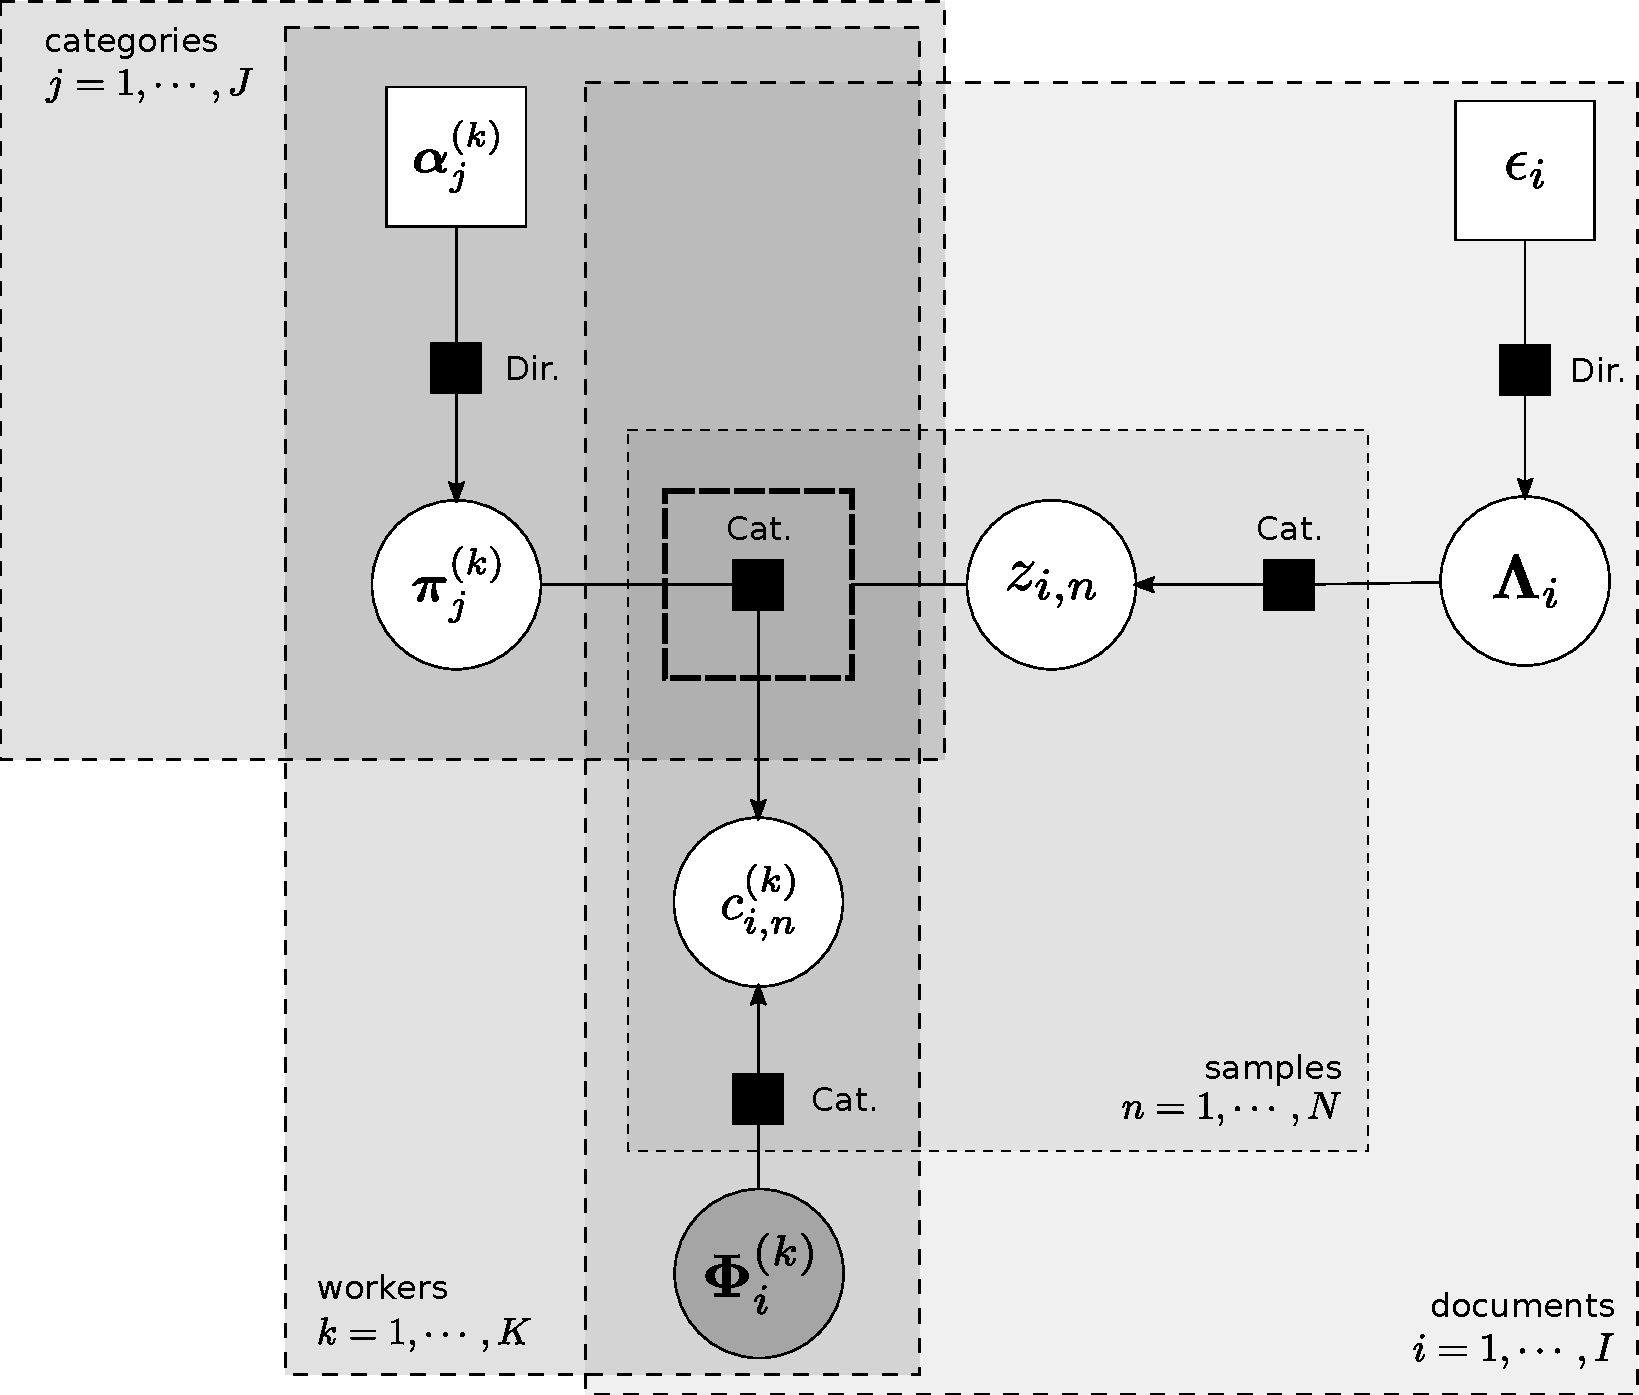
\includegraphics[scale=0.25]{res/m-bcc_fg}
\par\end{centering}

\protect\caption[Factor graph of MBCC.]{\label{fig:M-IBCC-FG}Factor graph of MBCC \cite{dietz_directed_2010}.}
\end{figure}



\section{Aggregating Judgments over Multiple Categories}

\label{sec:2-Model-Description}

Our proposed model -- referred to hereafter as multi-category independent
Bayesian classifier combination (MBCC) -- is a generalisation of
IBCC that deals with settings where documents have multiple categories.
\begin{algorithm}[t]
\begin{algorithmic}[1]

\scriptsize

\State{Input: the confusion matrices $\boldsymbol{\Pi}$ and the category proportions $\boldsymbol{\Lambda}$}

\State{}

\For{each document $i\in\left\{ 1,\cdots,I\right\}$}

\For{each sample $n\in\left\{ 1,\cdots,N\right\}$}
\State{Sample $z_{i,n}\sim \mbox{Cat}(\boldsymbol{\Lambda}_{i})$}
\For{each worker $k\in\left\{ 1,\cdots,K\right\}$}
\State{Sample $c_{i,n}^{(k)}\sim \mbox{Cat}\left(\boldsymbol{\pi}_{z_{i,n}}^{(k)}\right)$}
\EndFor
\EndFor

\State{}

\For{each worker $k\in\left\{ 1,\cdots,K\right\}$}
\For{each category $j\in\left\{ 1,\cdots,J\right\}$}

\State{$\Phi_{i,j}^{(k)} = \beta_{i,j}^{(k)} \sum_{n=1}^{N} \delta \left( c_{i,n}^{(k)} - j\right)$}
\State{where $\beta_{i,j}^{(k)}$ is a normalising constant.}
\EndFor
\EndFor

\EndFor

\State{}

\Return{$\boldsymbol{\Phi}$}
\end{algorithmic}

\protect\caption{\label{alg:MBCC-generative-process}Generative process of MBCC.}
\end{algorithm}
In more detail, we introduce a categorical distribution (i.e. the
category proportion) with parameter $\boldsymbol{\Lambda}_{i}$ over
the $J$ categories for each document $i$ (Equation \ref{eq:mbcc-p(z|)})
instead of the single categorical distribution $\boldsymbol{\kappa}$
common to all documents found in IBCC (Equation \ref{eq:ibcc-t|kappa}).
Moreover, each worker $k$
submits a distribution $\Phi_{i}^{(k)}$ over the $J$ categories
for each document $i$ instead of the single category $c_{i}^{(k)}$
required by IBCC. The confusion matrix $\boldsymbol{\Pi}^{(k)}$ of
each worker $k$ is kept unchanged from IBCC. Therefore in this new
setting, to assess the accuracy of each worker through their confusion
matrices $\boldsymbol{\Pi}^{(k)}$, we need to first independently
sample the aggregated distribution $\boldsymbol{\Lambda}_{i}$ to
obtain a set of categories $z_{i,n}$ for each document $i$ such
that 
\begin{equation}
z_{i,n}\sim\mbox{Cat}\left(\boldsymbol{\Lambda}_{i}\right),\label{eq:mbcc-p(z|)}
\end{equation}
for all samples $n\in\left\{ 1,\cdots,N\right\} $. The vector $\mathbf{z}_{i}$
of dimension $N$ can be seen as independent target categories $t_{i}$
of document $i$ (as in IBCC) drawn from the categories proportion
in Equation \ref{eq:mbcc-p(z|)}. We subsequently match these samples
against samples from each of the workers' distribution $\Phi_{i}^{(k)}$
to obtain 
\begin{equation}
c_{i,n}^{(k)}\sim\mbox{Cat}\left(\boldsymbol{\pi}_{z_{i,n}}^{(k)}\right)\label{eq:mbcc-p(c|)}
\end{equation}
for each document $i$. This is equivalent to running IBCC $N$ times
with different values of the workers' judgment $c_{i}^{(k)}$ drawn
from their distribution $\Phi_{i}^{(k)}$. In practice, one can perform
this sampling until the accuracy no longer increases. Alternatively,
a theoretical upper bound for an arbitrary level of error can be calculated
using Lemma 3 in \cite{devroye1983equivalence}. Thus, the joint
distribution is
\begin{multline}
p\left(\mathbf{z},\mathbf{c},\boldsymbol{\Lambda},\boldsymbol{\Pi}\right)=\prod_{i=1}^{I}\mbox{Cat}\left(\boldsymbol{\Lambda}_{i}\right)\mbox{Dir}\left(\epsilon_{i}\right)\times\\
\prod_{k=1}^{K}\prod_{n=1}^{N}\mbox{Cat}\left(\boldsymbol{\pi}_{z_{i,n}}^{(k)}\right)\prod_{j=1}^{J}\mbox{Dir}\left(\boldsymbol{\alpha}_{j}^{(k)}\right),\label{eq:mbcc-joint}
\end{multline}
where the hyperparameter $\nu$ in IBCC has been renamed for clarity
to $\epsilon_{i}$ (i.e. the pseudo-count of categories for each document
$i$), such that
\begin{equation}
\boldsymbol{\Lambda}_{i}\sim\mbox{Dir}\left(\epsilon_{i}\right).\label{eq:mbcc-p(lambda)}
\end{equation}


The generative process, that is, the random process by which MBCC
assumes the workers' judgment $\Phi_{i}^{(k)}$ arose, is summarised
in Figure \ref{fig:M-IBCC-FG} and Procedure \ref{alg:MBCC-generative-process}. In particular, we start
with the confusion matrices $\boldsymbol{\Pi}$, and the category
proportions $\boldsymbol{\Lambda}$ sampled from Equations \ref{eq:ibcc_p(pi|)}
and \ref{eq:mbcc-p(lambda)} respectively (Line 1). We then sample
$N$ categories $z_{i,n}$ from each category proportion $\boldsymbol{\Lambda}_{i}$
from Equation \ref{eq:mbcc-p(z|)} (Line 5). Given each category
$z_{i,n}$, we sample judgments $c_{i,n}^{(k)}$ from the workers'
$z_{i,n}$-th row of their confusion matrix $\boldsymbol{\Pi}^{(k)}$
(Line 7). Finally, we find the most likely categorical distributions
$\Phi_{i}^{(k)}$ which generated the samples $\mathbf{z}_{i}^{(k)}$
for all documents $i$ and workers $k$ (Line 13).





The key inferential problem that needs to be solved in order to use
MBCC is that of computing the posterior distribution of the latent
variables $\mathbf{z}$, and the parameters $\boldsymbol{\Lambda}$
and $\boldsymbol{\Pi}$ given the data $\mathbf{c}$, that is $p\left(\mathbf{z},\boldsymbol{\Lambda},\boldsymbol{\Pi}|\mathbf{c}\right)$.
 To do this, we can use approximation methods based on statistical
sampling (such as Markov chain Monte Carlo \cite{geman_stochastic_1984})
or density approximation (such as variational approximation \cite{jordan_introduction_1999,Attias00avariational}
or Laplace approximation \cite{laplace1986}). In particular, our
implementation uses the variational\emph{ }message passing algorithm
\cite{winn_variational_2005} as it has proven itself to be superior
in terms of speed and accuracy compared to both sampling and density
based approximation \cite{minka_expectation_2013}; but other approaches
could be used if appropriate. 


\section{Empirical Evaluation}

\label{sec:Empirical-Evaluation}

To evaluate the efficacy of our model, we use an independently gathered
dataset, and introduce two new datasets; all of which include ground
truth from expert annotators. We then compare performance against
four state-of-the-art benchmarks. The experiments are run in an
unsupervised setting, where the ground truth is never exposed to
the algorithms, and is only used to measure their accuracy. 
The source code and datasets are available at \cite{augustin_mbcc_2017}.


\subsection{Datasets}

\label{sub:4.1-Dataset}





Our experiments use a total of three datasets. 

\textbf{SemEval.} This dataset contains judgments of sentiments
within one hundred news headlines sampled from the SemEval2007 test
set \cite{strapparava_semeval-2007_2007,snow_cheap_2008}. Each
worker was presented with a list of headlines, and was asked to give
numeric judgments between zero and a hundred for each of six sentiments.
Ten judgments were collected for each headline for a total of 1,000
judgments. These judgments were obtained from 38 workers whom provided
a minimum of 20 judgments each, and 26 on average. We truncate
the total number of judgments per worker to 20 to avoid discrepancies
in accuracy of each inferred confusion matrix. We normalise the
values submitted by each worker into valid probability distributions
by ensuring that the total area is equal to one at any given time.\textbf{} 

\textbf{IAPR-TC12.} We crowdsourced a set of 16 images sampled
from the IAPR-TC12 dataset \cite{escalante_segmented_2010,augustin_mbcc_2017}.
This is a collection of 20,000 images of urban and rural scenes
manually segmented per regions. Each pixel belongs to one of six
region. We gathered a total of 16 judgments per image from 21
workers. Workers were asked to estimate the proportion of each
region in the image. The ground truth proportion for each category
is calculated by dividing the number of pixels in the region by the
total number of pixels in the image. The workers reported their judgments
with a pie chart, enabling quick and accurate judgments of proportion
\cite{hollands_judgments_1992}. 

\textbf{Colours}. We crowdsourced a set of 460 judgments of the
proportion of colours in the flags of 20 countries \cite{augustin_mbcc_2017}.
We asked 23 participants to judge, from memory, the proportion of
10 colours in each country's flag. 

\textbf{} The alternatives in each dataset are complete, that
is, using all the categories can always fully describe the instance.
Furthermore, although these three datasets may already contain spammers,
we augment the datasets with additional synthetic spammers to explore
the loss of accuracy as they increase in number. Vuurens et al. \cite{vuurens_how_2011}
identified four types of spammers: sloppy, uniform, random and semi-random.
While sloppy workers try to the best of their abilities to complete
the tasks, they may be insufficiently precise in their judgments.
On the other hand, uniform spammers use a fixed uniform judgment pattern
across all documents. Finally, random spammers provide unique meaningless
answers for each document and semi-random spammers also answer a
few questions properly. While the obvious characteristic of repeating
judgment patterns can be used to manually filter out uniform spammers,
random spammers are the most challenging to detect. For this reason,
we use a random spamming strategy where a spammer always provides
a random categorical distribution for each document. The distribution
of each spammer $k$ for each document $i$ shares a prior Dirichlet
distribution such that
\begin{equation}
\Phi_{i}^{(k)}\sim\mbox{Dir}\left(\mathbf{1}\right),\label{eq:spammer-prior}
\end{equation}
where the pseudo-count of $\mathbf{1}$ ensures that all possible
distributions $\Phi_{i}^{(k)}$ are equally likely.


\subsection{Experimental Setting}

\label{sub:4.2-Experimental-Setting}



\begin{figure*}[t]
\begin{centering}
\subfloat{\protect\centering{}\label{fig:error_vs_spammers_semeval}\protect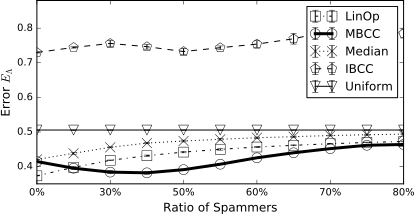
\includegraphics[scale=0.57]{res/semeval2007_error_vs_spammers}\protect}\hfill{}\subfloat{\protect\centering{}\label{fig:error_vs_samples_semeval}\protect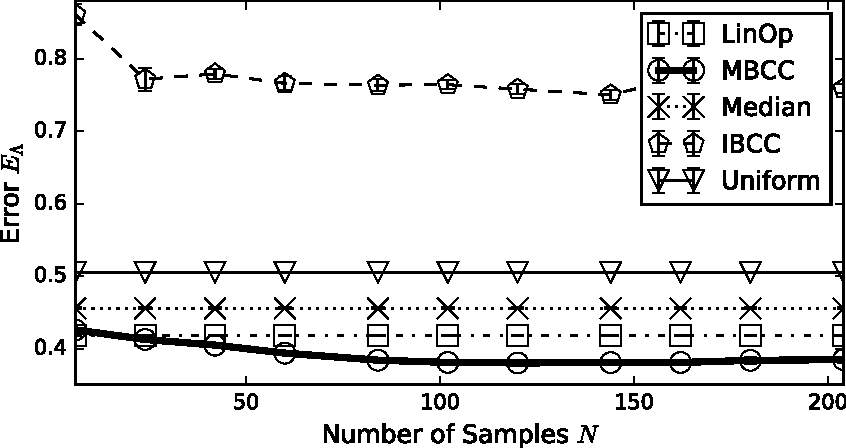
\includegraphics[scale=0.57]{res/semeval2007_error_vs_samples}\protect}
\par\end{centering}

\protect\caption{\label{fig:semeval}Average error on the aggregated distributions
$\boldsymbol{\Lambda}$ on the SemEval dataset when increasing: (left)
the ratio of spammers at $N=180$ samples, (right) the number of samples
at a ratio of spammers of 50\%. }
\end{figure*}


\begin{figure*}[t]
\begin{centering}
\subfloat{\protect\centering{}\label{fig:error_vs_spammers_image_seg}\protect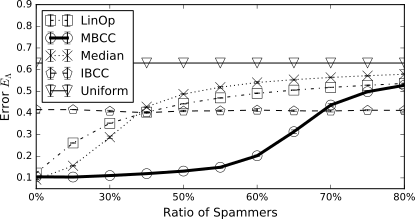
\includegraphics[scale=0.57]{res/sbd_error_vs_spammers}\protect}\hfill{}\subfloat{\protect\centering{}\label{fig:error_vs_spammers_flags}\protect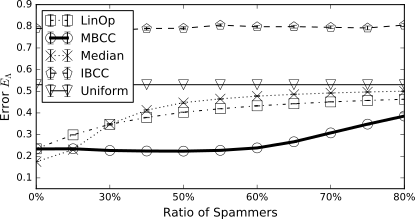
\includegraphics[scale=0.57]{res/flags_10_error_vs_spammers}\protect}
\par\end{centering}

\protect\caption{\label{fig:error_vs_spammers}Average error on the aggregated distributions
when increasing the ratio of spammers on: (left) the IAPR-TC12 dataset
at $N=180$ samples, (right) the Colours dataset at $N=330$ samples.}
\end{figure*}








\textbf{}We set the parameter of the prior probability of each
confusion matrix for all workers and spammers to $\mathbf{A}^{(k)}=100\times\mathbf{I}+\mathbf{1}^{T}\mathbf{1}$.
This means that workers are initially assumed to be reasonably accurate
before seeing any data. Using a different assumption leads to distinct
aggregation accuracy profiles that will be discussed in more detail
in Section \ref{sub:4.5-Results}. Furthermore, to ensure fair comparison
between the benchmarks, we do not adjust each parameters $\boldsymbol{\epsilon}$
of the prior distributions over categories to reflect the balance
of each dataset.\textbf{} Finally, we run all models a hundred
times each to achieve statistically significant results at the 99\%
confidence level.


\subsection{Benchmarks}

\label{sub:4.3-Benchmarks}

We compare the performance of our model to four state of the art
benchmark methods.

\textbf{Uniform }assigns a uniform distribution for each aggregated
distribution (i.e. $p_{j}=\frac{1}{J}$ for all $j\in\left\{ 1,\cdots,J\right\} $),
making it independent of the dataset. These particular values of
$p_{j}$ maximise the entropy function of categorical distributions.
That is, if one were to guess the aggregated distribution far from
the ground truth on average (given some distance metric), it can
be expected to have its error above the uniform model.  

\noindent \indent \textbf{LinOp }averages the distributions
provided by the workers. Unlike IBCC and MBCC, it does not sample
the workers' distributions to produce the discrete observations, but
directly takes the distributions as input.  As there is no training
set for assigning informative weights to the workers, we assign equal
weights $\omega^{(k)}=\frac{1}{K}$ to each worker.

\noindent \indent \textbf{Median }estimates the aggregated distribution
by arranging the judgments for each document in ascending order
and then takes the middle judgment. Each judgment is considered with
equal weight for the same reason as for LinOp. The median is a robust
method against extreme judgements since it will not give an arbitrarily
large or small result if no more than half of the judgments for a
document are incorrect.





\noindent  

\noindent \indent \textbf{IBCC}  combines discrete judgments
from multiple workers and models the ability of each individual worker
using confusion matrices \cite{kim_bayesian_2012}. Although IBCC
takes a single category as ground truth, the output is a posterior
distribution over the categories which can be compared to the ground
truth category proportion.

\noindent 


\subsection{Accuracy Metrics}

\label{sub:4.4-Accuracy-Metric}



To assess the accuracy of the inference, we use the Euclidean distance.
Specifically, we define the average error of the aggregation on the
entire dataset by 
\begin{equation}
E_{\boldsymbol{\Lambda}}=\frac{1}{I}\sum_{i=1}^{I}\mathrm{d}\left(\boldsymbol{\Lambda}_{i}^{*},\boldsymbol{\Lambda}_{i}\right)\label{eq:error-dist}
\end{equation}
where $\mathrm{d}\left(.\right)$ is the Euclidean distance, $I$
the total number of documents, $\boldsymbol{\Lambda}_{i}^{*}$
the ground truth distribution for document $i$, and $\boldsymbol{\Lambda}_{i}$
the aggregated distribution provided by the model for document $i$.
Furthermore, we define the deviation of the confusion matrix $\boldsymbol{\Pi}^{(k)}$
of worker $k$ to the identity matrix $\mathbf{I}$ by 
\begin{equation}
E_{\boldsymbol{\Pi}^{(k)}}=\sum_{j=1}^{J}\mathrm{d}\left(\mathbf{I}_{j},\boldsymbol{\pi}_{j}^{(k)}\right).\label{eq:error-cm}
\end{equation}
Other distance metric can be used, provided that it gives finite
results when the distributions are not absolutely continuous. 
\begin{figure}[t]
\begin{centering}
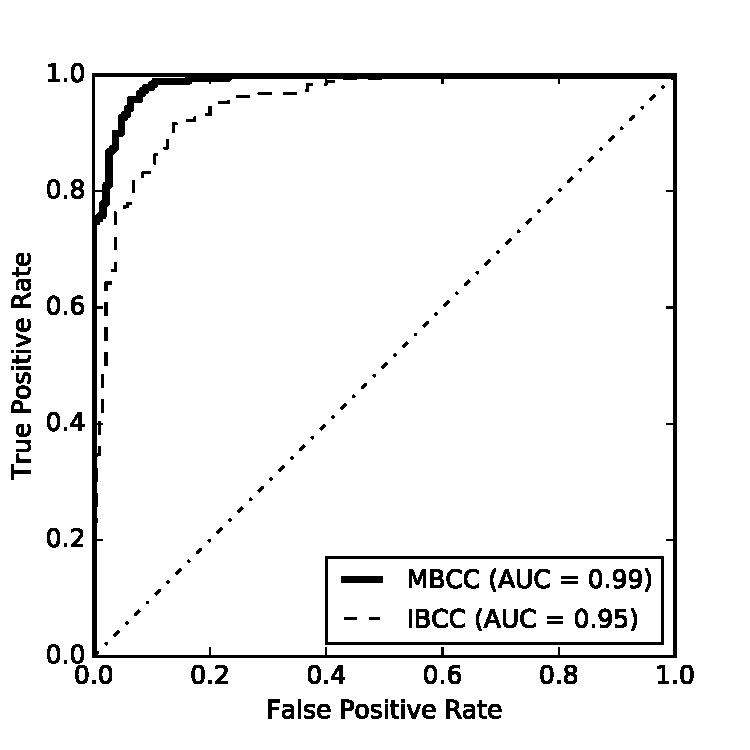
\includegraphics[scale=0.48]{res/semeval2007_roc_sr_1}
\par\end{centering}

\protect\caption{\label{fig:ROC}ROC curves on the SemEval dataset. The ratio of spammers
is set to 50\%. }
\end{figure}



\subsection{Results}

\label{sub:4.5-Results}



We now present the results of our empirical evaluation regarding a
number of key aspects: (i) accuracy of aggregation and robustness
to spammers, (ii) convergence and running time, (iii) classification
of spammers.  We first consider  in detail the results on the SemEval
dataset, and briefly discuss the results on the other datasets.

Figure \ref{fig:semeval} (left) shows the average error as the
ratio of spammers increases on the SemEval dataset.  To illustrate,
a ratio of spammers of 50\% means half the workers in the dataset
are spammers. As can be seen, MBCC achieves a comparable aggregation
accuracy when 50\% of the workers are spammers, as LinOp does when
no spammers are added. However, the added complexity of detecting
spammers in MBCC comes at a cost when the level of spammers is low.
Indeed, the highest precision is initially produced by LinOp, but
as the ratio of spammers increases a crossover point is reached after
which MBCC is the most precise. The value of this crossover point
can be adjusted by varying the pseudo-counts of prior observations
$\mathbf{A}_{ii}^{(k)}$ on the diagonal of the workers' confusion
matrix. For high values, MBCC assumes all workers are truthful.
This is the assumption underpinning LinOp, where all workers have
an implicit identity matrix as their confusion matrix. In fact, for
high pseudo-counts, the performance of MBCC matches perfectly with
LinOp regardless of the number of spammers. On the other hand, with
lower values of pseudo-counts, MBCC allows greater flexibility to
learn the spammers, at the cost of having a greater error when there
are fewer spammers in the dataset. Therefore, the added degrees of
freedom lead to a tradeoff in accuracy at different ratio of spammers.
Furthermore, we set the number of samples $N$ empirically. Figure
\ref{fig:semeval} (right) shows the average error of the aggregated
distribution when increasing the number of samples at a ratio of
spammers of 50\%. As the number of samples increases, we observe
convergence of the error at 100 samples to values of 0.75 and 0.37
for IBCC and MBCC respectively. Inevitably, the running time also
increases as the number of samples increases.  In particular, the
running time of LinOp and Median is typically 3ms, while that of
IBCC and MBCC ranges from 12s and 13s, to 6min and 28min respectively,
across the range of samples shown in Figure \ref{fig:semeval} (right).


We now evaluate the accuracy of the confusion matrix-based models
at classifying workers from spammers on the SemEval dataset. To do
this, we first collect the inferred confusion matrix $\boldsymbol{\Pi}^{(k)}$
for each worker. We then compute the deviation $E_{\mathbf{\Pi}^{(k)}}$
of each confusion matrix to the identity matrix (Equation \ref{eq:error-cm}).
The identity matrix represents the confusion matrix of a perfect worker,
that is, one that always gives judgments in accordance with the consensus.
We then set a threshold on the error, above which a worker is classified
as a spammer.    The receiver operating characteristic (ROC) curves
in Figure \ref{fig:ROC} capture the effect of varying the threshold
of the error. As can be seen, MBCC has an area under the curve (AUC)
of 0.99, showing a 5 times improvement compared to IBCC in terms
of the expected number of misclassified spammers.  The AUC eventually
decreases for both models at higher ratios. 

We now briefly discuss the results on the two other datasets. On
the IAPR-TC12 dataset (Figure \ref{fig:error_vs_spammers} (left)),
LinOp, Median and MBCC achieve equal accuracies when no spammers
are added. However, since each image in this dataset is dominated
by a single category, that is, at least one category has more than
50\% coverage in each image, IBCC performs reasonably well even with
a high ratio of spammers. This is because IBCC always assigns a
probability of one to the most likely category, which emphasises its
assumption that documents have exactly one category. In fact, as
the documents' proportion regresses to Kronecker deltas, the error
from IBCC decreases. On the Colours dataset (Figure \ref{fig:error_vs_spammers}
(right)), the accuracy of MBCC remains a lower bound of LinOp throughout
the range of ratios of spammers. However, Median initially achieves
the lowest error with a crossover point with MBCC at 15\% spammers.
This is because the judgments provided by the workers include sufficient
outliers, making the Median a good measure of central tendency.
Finally, convergence of the error on the aggregation is reached
at 100 samples for the IAPR-TC12 dataset and 150 for the Colours dataset.
Since the Colour dataset has 4 more categories than the IAPR-TC12
datasets, it requires more samples to achieve convergence.  






\section{Conclusions}

\label{sec:5-Conclusions}

We introduced a novel model for the aggregation of categorical distributions.
The key innovations of our method are the elicitation and sampling
of judgments of proportions in the form of probability distributions
and the use of these samples to improve on the accuracy of aggregation.
In particular, we showed empirically, on three real-world datasets,
that our approach outperforms existing methods by up to 28\% in terms
of accuracy. We have also shown a comparable level of accuracy when
60\% of the workers are spammers, as other approaches do when there
are no spammers. Finally, we improved the expected number of misclassified
spammers by up to five times that achieved by existing methods. 
 

\bibliographystyle{named}
\bibliography{ijcai17}





\end{document}
